% vim:ft=tex

\section{Pelias}
\subsection{General}
\subsubsection{Capabilities}
Pelias is a software solution/library used for geocoding. Geocoding is the process of taking input text, such as an address or the name of a place and returning a latitude/longitude location on the Earth's surface for that place.
The "senior team" used Nominatim for geocoding, which is a tool for geocoding just like pelias. One of our main tasks  in the course of the first half of the project was to test and evaluate pelias as an alternative open-source geocoder to Nominatim.

Here are some benefits of the pelias API:
\begin{itemize}
\item Completely open-source and MIT licensed
\item A powerful data import architecture: Pelias supports many open-data projects out of the box but also works great with private data
\item Support for searching and displaying results in many languages
\item Fast and accurate autocomplete for user-facing geocoding
\item Support for many result types: addresses, venues, cities, countries, and more
\item Easy installation with minimal external dependencies
\end{itemize}

As mentioned above, pelias has the ability to import data from many different open-data projects as well as own private data. The importers filter, normalize, and ingest geographic datasets into the Pelias database. Currently there are five officially supported importers:

\begin{itemize}
\item \textbf{OpenStreetMap:} supports importing nodes and ways from OpenStreetMap
\item \textbf{OpenAddresses:} supports importing the hundreds of millions of global addresses collected from various authoritative government sources by OpenAddresses
\item \textbf{Who's on First:} supports importing admin areas and venues from Who's on First
\item \textbf{Geonames:} supports importing admin records and venues from Geonames
\item \textbf{Polylines:} supports any data in the Google Polyline format. It's mainly used to import roads from OpenStreetMap
\item \textbf{Custom Data Importer:} creates a Pelias record for each row in a CSV file. Each row must define a source, latitude, longitude, and either an address, name, or both. This feature was used to import two-digit postcodes into Pelias.
\end{itemize}

\begin{figure}[H]
\centering
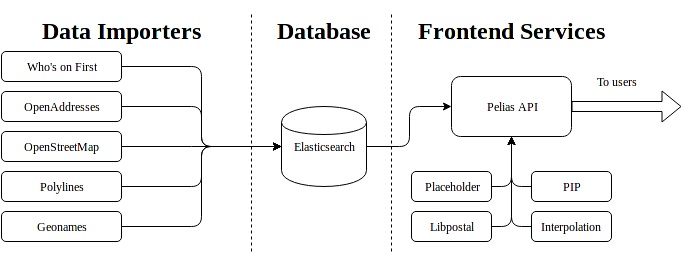
\includegraphics[width=1.0\textwidth]{img/pelias_architecture}
\captionof{figure}{Overview of the pelias architecture}
\label{fig:pelias_architecture}
\end{figure}

\subsubsection{Database}
The underlying datastore that powers the search results and does query-lifting is Elasticsearch. Currently version 2.4 is supported, with plans to support 5.x soon. The developers built a tool called pelias-schema that sets up Elasticsearch indices properly for Pelias.

\subsubsection{Dependencies}
These are software projects that are not used directly but are used by other components of Pelias:
\begin{itemize}
\item \textbf{model:} provide a single library for creating documents that fit the Pelias Elasticsearch schema. This is a core component of Pelias‘ flexible importer architecture
\item \textbf{wof-admin-lookup:} A library for performing administrative lookup using point-in-polygon math. Previously included in each of the importers but now only used by the PIP service.
\item \textbf{query:} This is where most of Elasticsearch’s query generation happens.
\item \textbf{config:} Pelias is very configurable, and all of it is driven from a single JSON file which is called pelias.json. This package provides a library for reading, validating, and working with this configuration. It is used by almost every other Pelias component
\item \textbf{dbclient:} A Node.js stream library for quickly and efficiently importing records into Elasticsearch
\end{itemize}

\subsection{System Requirements}
\subsubsection{Software Requirements}
\begin{itemize}
\item \textbf{Node.js:} Version 8 or newer is required, version 10 is recommended for improved performance.
\item \textbf{Elasticsearch:} Version 2.4 or 5.6
\item \textbf{SQLite:} Version 3.11 or newer
\item \textbf{Libpostal:} Pelias relies heavily on the Libpostal address parser. Libpostal requires about 4GB of disk space to download all the required data.
\end{itemize}

\subsubsection{Hardware Requirements}
\begin{itemize}
\item At a minimum 50GB disk space to download, extract, and process data
\item 8GB RAM for a local build, 16GB+ for a full planet build. Pelias needs a little RAM for Elasticsearch, but much more for storing administrative data during import
\item As many CPUs as possible. There's no minimum, but Pelias builds are highly parallelizable, so more CPUs will help make it faster.
\end{itemize}

Actual system used for the project (Europe build):
\begin{itemize}
\item 1 virtual machine (Ubuntu Linux) with 64 GB RAM, 500GB HDD, 4 CPU cores
5
\item RAM utilization is at ~30 GB, however during the import of openstreetmaps data and calculating polylines from it up to 40 GB of RAM were used. Imports and calculations maxed out all CPU cores. It is possible to reduce the required amount of RAM for imports and calculations. However, this requires splitting up openstreetmap files in smaller files with other tools beforehand.
\item Including “raw data” (before the import and calculations) around 400GB of data are persisted on HDD, Elasticsearch uses ~100GB.
\end{itemize}